% !TeX program = pdflatex
\documentclass[11pt]{article}
\usepackage[a4paper,margin=1in]{geometry}
\usepackage{times}
\usepackage{hyperref}
\usepackage{graphicx}
\usepackage{tikz}
\usetikzlibrary{arrows.meta,positioning,shapes,fit}
\usepackage{listings}
\usepackage{caption}
\usepackage{subcaption}
\usepackage{booktabs}
\usepackage{amsmath,amssymb}
\usepackage{xcolor}

\title{Plan-Driven, Tool-First Retrieval Augmented Generation for Building Analytics\\A Practical System with Hybrid Retrieval, Chart Planning, and Reliable Visualization}
\author{AVMSolutions Team}
\date{\today}

\begin{document}
\maketitle

\begin{abstract}
We present a production-grade Retrieval Augmented Generation (RAG) system for building analytics that combines: (i) hybrid retrieval (sparse + vector + reranker) tuned for scientific/technical language, (ii) a tool-first agent that converts plot intents to a validated chart plan before generation, and (iii) robust visualization with dataRef resolution, schema checks, and shape-preserving downsampling. We formalize the pipeline stages (pre-retrieval, retrieval, post-retrieval, augmentation, and generation), provide design rationales grounded in recent surveys \cite{zhao2024rag-survey} and hybrid systems \cite{yuan2024hybrid-crag}, and specify component-level evaluation. Our system emphasizes reliable, grounded charts (heatmaps, histograms, stacked/area, dual-axis overlays, forecasts with confidence bands), adaptive retrieval depth (L1--L4), and a production posture suitable for AWS deployments. We report a benchmark harness capable of auto-generating figures and tables from end-to-end runs, and propose a transparent test matrix to compare against conventional RAG variants and ablate major design choices.
\end{abstract}

\section{Introduction}
\label{sec:intro}
RAG augments LLMs with external data to improve factuality, timeliness, and controllability. However, many real systems struggle with (a) retrieval quality under domain-specific language, (b) unreliable plotting where LLMs hallucinate data arrays, and (c) missing guardrails that degrade UX in enterprise settings. We target building analytics (indoor environment/IAQ, occupancy, energy), a domain mixing scientific vocabulary and time-series numerics.

This paper contributes: (1) a \emph{plan-driven, tool-first} RAG agent that always grounds charts via dataRef and validated tool outputs; (2) a \emph{hybrid retrieval} stack (BM25/TF--IDF + Sci-domain sentence embeddings + SBERT reranker) with query-level adaptive depth; (3) \emph{reliable charting} with schema validation and Largest-Triangle-Three-Buckets (LTTB) downsampling; and (4) a \emph{comprehensive evaluation protocol} contrasting standard RAG baselines. Our design aligns with best practices summarized in \cite{zhao2024rag-survey} and integrates hybrid reasoning enhancements in the spirit of \cite{yuan2024hybrid-crag}.

\section{Background and Related Work}
\label{sec:related}
\paragraph{RAG foundations.} Retrieval Augmented Generation augments LLMs with external context. Zhao et al.\ \cite{zhao2024rag-survey} survey techniques across the full stack, advocate query-level stratification (L1--L4), and emphasize hybrid retrieval with reranking.

\paragraph{Hybrid retrieval and reranking.} Hybrid fusion (RRF) blends sparse (lexical) and dense (semantic) retrieval. Lightweight rerankers (SBERT) improve top-$M$ precision. Xu et al.\ \cite{xu2025ragwild} report that in mixture-of-knowledge settings, rerankers may add marginal value and retrieval benefits diminish for stronger backbones, motivating adaptive retrieval and robust augmentation.

\paragraph{Complex reasoning.} Yuan et al.\ \cite{yuan2024hybrid-crag} report comprehensive enhancements for complex reasoning tasks. We adapt those insights to measurement-heavy building analytics with reliable visualization.

\paragraph{Reliable visualization.} We enforce dataRef-only charts, plan-first construction, and runtime validation to avoid LLM-created array hallucinations.

\paragraph{Evaluation.} We combine retrieval metrics (Recall@k, nDCG, MRR), RAGAS-style metrics (answer relevancy, context recall/precision, faithfulness), and chart-centric metrics (schema success, intent, fidelity, latency). Our harness is designed to reflect challenges observed in \cite{xu2025ragwild} (e.g., heterogeneous corpora, variable gains across backbones).

\section{System Overview}
\label{sec:overview}
Figure~\ref{fig:pipeline} sketches the pipeline:
\begin{enumerate}
  \item \textbf{Pre-Retrieval:} Document building and chunking, table extraction, vectorization.
  \item \textbf{Retrieval:} Hybrid sparse + vector retrieval; RRF fusion; lexical nudging; SBERT reranker for top-$M$.
  \item \textbf{Post-Retrieval:} Re-ranking, filtering, deduplication; building concise, schema-aware context.
  \item \textbf{Augmentation:} Tool-first agent compiles a chart plan (\texttt{chart\_query}); tools are executed; dataRefs are resolved.
  \item \textbf{Generation:} Final answer + validated chart (schema checks, LTTB downsampling, Vega-Lite fallback).
\end{enumerate}

\begin{figure}[t]
  \centering
  % Simple TikZ schematic (self-contained)
  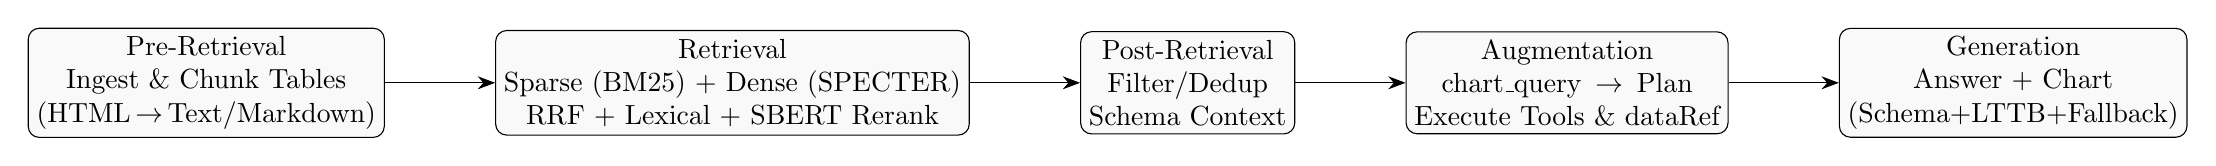
\begin{tikzpicture}[
    node distance=10mm and 14mm,
    box/.style={draw, rounded corners, align=center, inner sep=3pt, fill=gray!5},
    >={Stealth[length=2.2mm]}
  ]
  \node[box] (ingest) {Pre-Retrieval\\Ingest \& Chunk Tables\\(HTML\,$\to$\,Text/Markdown)};
  \node[box, right=of ingest] (retr) {Retrieval\\Sparse (BM25) + Dense (SPECTER)\\RRF + Lexical + SBERT Rerank};
  \node[box, right=of retr] (post) {Post-Retrieval\\Filter/Dedup\\Schema Context};
  \node[box, right=of post] (augment) {Augmentation\\chart\_query \,$\to$\, Plan\\Execute Tools \& dataRef};
  \node[box, right=of augment] (gen) {Generation\\Answer + Chart\\(Schema+LTTB+Fallback)};
  \draw[->] (ingest) -- (retr);
  \draw[->] (retr) -- (post);
  \draw[->] (post) -- (augment);
  \draw[->] (augment) -- (gen);
  \end{tikzpicture}
  \caption{System schematic: plan-driven RAG pipeline.}
  \label{fig:pipeline}
\end{figure}

\section{Pre-Retrieval}
\label{sec:pre}
\subsection{Data Ingestion and Chunking}
\textbf{Text:} HTML parsing, boilerplate removal, sentence segmentation, question/answer-aware chunk grouping.\
\textbf{Tables:} Extract to Markdown; preserve structure for later retrieval and numeric reasoning.

\subsection{Indexing}
\textbf{Sparse:} TF--IDF/BM25 for exact-term recall.\
\textbf{Dense:} Sentence-Transformers (default: SPECTER) for scientific semantics.\
\textbf{Why hybrid?} Matches domain synonyms and nomenclature while keeping lexical precision.

\section{Retrieval}
\label{sec:retrieval}
\subsection{Fusion and Reranking}
\textbf{RRF:} Reciprocal Rank Fusion blends sparse and dense lists.\
\textbf{Lexical nudging:} Adds explicit-overlap score.\
\textbf{SBERT reranker:} Python sidecar reranks top-$M$ by semantic similarity (same model family as embeddings).

\subsection{Adaptive Depth by Query Level}
L1--L4 vary top-$k$ to balance latency and recall (e.g., L1=8, L4=24). This mirrors L1--L4 stratification advocated by \cite{zhao2024rag-survey}.

\section{Post-Retrieval}
\label{sec:post}
\subsection{Filtering and Consolidation}
Remove near-duplicates, low-signal chunks, and misaligned snippets; summarize long tables/text as needed.

\subsection{Schema-Aware Context}
Include room/table schemas and time windows to steer tools (field and table inference). This lowers LLM friction.

\section{Augmentation}
\label{sec:augment}
\subsection{Plan-Driven Chart Construction}
\textbf{chart\_query:} Converts plot intent into a tool \emph{plan} plus Highcharts options with \emph{dataRef}. Tools are executed; dataRefs are resolved to actual series. No embedded arrays.

\subsection{Validation and Reliability}
\textbf{Schema checks:} Enforce series+dataRef presence, tool existence; error out early.\
\textbf{Downsampling:} LTTB preserves shape for large series.\
\textbf{Fallback:} Vega-Lite \textrightarrow{} Highcharts conversion for resilience.

\section{Generation}
\label{sec:generation}
\subsection{Tool-First Agent}
LLM is free to reason but bound to tools for data; tool arguments are steered from the question (e.g., humidity \textrightarrow{} iaq.humidity). Plot intents can be auto-served without LLM chart freeform.

\subsection{Robust Chart Types}
Line/area (stacked), scatter (paired), histogram, heatmap (correlation), dual-axis overlays, forecast with CI bands.

\section{Evaluation Protocol}
\label{sec:evaluation}
\subsection{L1--L4 Query Examples and Handling}
\begin{itemize}
  \item \textbf{L1 (Explicit facts):} ``What is the latest CO$_2$ value in B\_F3\_lab?''\\
  Retrieval (small $k$), tool: \texttt{latest\_value(iaq, co2)}, generate concise answer.
  \item \textbf{L2 (Implicit facts):} ``Compare average humidity across labs this week.''\\
  Hybrid retrieval ($k$ larger), tools: \texttt{compare\_rooms\_on\_metric(iaq, humidity, agg=avg)}; chart via dataRef bar.
  \item \textbf{L3 (Interpretable rationale):} ``Is ventilation sufficient by guideline X?''\\
  Retrieve guideline passages; compute CO$_2$ compliance via tools; generate rationale citing thresholds.
  \item \textbf{L4 (Hidden rationale):} ``Why did energy peak on Tue 3pm?''\\
  Multi-hop retrieval (larger $k$), correlate \texttt{energy} with \texttt{people/weather}; pairwise tools; reason aggregated evidence.
\end{itemize}

\subsection{Retrieval Metrics}
Recall@k, nDCG@k, MRR on labeled query sets; human graded relevance for domain language. Compare: sparse-only, dense-only, hybrid, hybrid+rerank.

\subsection{Augmentation/Chart Reliability}
\textbf{Chart success rate:} (valid schema, data present) first-pass.\
\textbf{Fidelity:} LTTB vs uniform vs none (DTW/EMD similarity; human preference).\
\textbf{Intent correctness:} fraction of plots matching requested metric/table.

\subsection{End-to-End QA}
Exact match / F1 where available; human evaluation for factuality and hallucinations (penalize wrong confident answers).

\subsection{Ablations}
Remove/replace: reranker, LTTB, dataRef enforcement, auto plot-intent handling, SBERT model variants. Report accuracy/latency deltas.

\subsection{Comparison Tables (from Bench Harness)}
% Auto-generated tables (chart reliability) will be written to results/tables.tex by scripts/bench/gen_tex.py
% Auto-generated tables from bench runs
\begin{table}[h]
  \centering
  \caption{Chart reliability summary across runs (this system).}
  \begin{tabular}{lcccc}
    \toprule
    Run & Cases & Chart Succ. & Intent OK & p95 Latency (s)\\\midrule
    20251021T000755Z & 15 & 93.3\% & 73.3\% & 42.9949164390564\\
    \bottomrule
  \end{tabular}
\end{table}


\subsection{Answer Quality (from Bench Harness)}
% Auto-generated Answer Quality table (with references) is written to results/answers.tex by scripts/bench/score_answers.py
% Answer quality metrics (reference-based, provider-agnostic)
\begin{table}[h]
  \centering
  \caption{Answer quality over bench cases (Exact, Token F1, ROUGE-L, Numeric).}
  \begin{tabular}{lcccc}
    \toprule
    Cases & Exact & Token F1 & ROUGE-L & Numeric \\ \midrule
    15 of 15 & 0.000 & 0.137 & 0.120 & 0.163 \\
    \bottomrule
  \end{tabular}
\end{table}


\subsection{Answer Faithfulness (No-Reference)}
% Auto-generated reference-free table is written to results/answers_noref.tex by scripts/bench/score_answers_noref.py
% Reference-free answer faithfulness metrics
\begin{table}[h]
  \centering
  \caption{Reference-free answer evaluation: grounding precision, intent coverage, plausibility penalty.}
  \begin{tabular}{lccc}
    \toprule
    Cases & Grounding & Intent & Plausibility \\ \midrule
    15 & 0.400 & 0.774 & 0.236 \\
    \bottomrule
  \end{tabular}
\end{table}


\subsection{Bench Figures}
% Auto-generated figure includes (latest run) are written to results/images.tex by scripts/bench/gen_images_tex.py
% Auto-generated image includes for latest run
% Run: 20251021T000755Z
\begin{figure}[h]
  \centering
  \begin{subfigure}[b]{0.49\linewidth}
    
\includegraphics[width=\linewidth]{docs/publication/figures/20251021T000755Z/heatmap_corr_lab.png}
    \caption{Model}
  \end{subfigure}
  \begin{subfigure}[b]{0.49\linewidth}
    
\includegraphics[width=\linewidth]{docs/publication/figures/20251021T000755Z/heatmap_corr_lab_ref.png}
    \caption{Reference}
  \end{subfigure}
  \caption{heatmap corr lab}
\end{figure}
\begin{figure}[h]
  \centering
  \begin{subfigure}[b]{0.49\linewidth}
    
\includegraphics[width=\linewidth]{docs/publication/figures/20251021T000755Z/histogram_lux_lab.png}
    \caption{Model}
  \end{subfigure}
  \begin{subfigure}[b]{0.49\linewidth}
    
\includegraphics[width=\linewidth]{docs/publication/figures/20251021T000755Z/histogram_lux_lab_ref.png}
    \caption{Reference}
  \end{subfigure}
  \caption{histogram lux lab}
\end{figure}
\begin{figure}[h]
  \centering
  
\includegraphics[width=0.86\linewidth]{docs/publication/figures/20251021T000755Z/l1_latest_co2.png}
  \caption{l1 latest co2}
\end{figure}
\begin{figure}[h]
  \centering
  
\includegraphics[width=0.86\linewidth]{docs/publication/figures/20251021T000755Z/l1_latest_humidity.png}
  \caption{l1 latest humidity}
\end{figure}
\begin{figure}[h]
  \centering
  
\includegraphics[width=0.86\linewidth]{docs/publication/figures/20251021T000755Z/l1_latest_temperature.png}
  \caption{l1 latest temperature}
\end{figure}
\begin{figure}[h]
  \centering
  \begin{subfigure}[b]{0.49\linewidth}
    
\includegraphics[width=\linewidth]{docs/publication/figures/20251021T000755Z/l2_daily_co2_compare.png}
    \caption{Model}
  \end{subfigure}
  \begin{subfigure}[b]{0.49\linewidth}
    
\includegraphics[width=\linewidth]{docs/publication/figures/20251021T000755Z/l2_daily_co2_compare_ref.png}
    \caption{Reference}
  \end{subfigure}
  \caption{l2 daily co2 compare}
\end{figure}


\subsection{Comparison Tables (Placeholders)}
\begin{table}[h]
  \centering
  \caption{Retrieval variants vs metrics (placeholder).}
  \begin{tabular}{lcccc}
    \toprule
    Variant & Recall@10 & nDCG@10 & MRR & Latency (ms)\\\midrule
    Sparse only & -- & -- & -- & --\\
    Dense only & -- & -- & -- & --\\
    Hybrid (RRF+lex) & -- & -- & -- & --\\
    Hybrid + rerank & -- & -- & -- & --\\\bottomrule
  \end{tabular}
  \label{tab:retrieval}
\end{table}

\begin{table}[h]
  \centering
  \caption{Chart reliability (success/fidelity) vs settings (placeholder).}
  \begin{tabular}{lccc}
    \toprule
    Setting & Chart success \% & Fidelity (DTW) & Time (ms)\\\midrule
    No sampling & -- & -- & --\\
    Uniform sampling & -- & -- & --\\
    LTTB sampling & -- & -- & --\\\bottomrule
  \end{tabular}
  \label{tab:charts}
\end{table}

\section{Tool Usage Examples}
\label{sec:tools}
\subsection{chart\_query Request/Response}
\begin{lstlisting}[language=json, basicstyle=\ttfamily\small, caption={chart\_query example (daily humidity, combined).}]
{
  "tool": "chart_query",
  "args": {
    "intent": "Daily average humidity across two rooms with combined line",
    "metric": "humidity",
    "rooms": ["B_F3_lab", "B_F3_toilet"],
    "granularity": "daily"
  }
}
\end{lstlisting}
\noindent Returns plan (\texttt{daily\_avg\_across\_rooms}) and a Highcharts object with dataRef; the agent executes the plan and resolves series.

\subsection{Tool Calls with dataRef}
\begin{lstlisting}[language=json, basicstyle=\ttfamily\small, caption={Histogram and heatmap chart specs with dataRef.}]
{
  "chart": {"type": "column"},
  "series": [{
    "name": "Lab lux histogram",
    "dataRef": {"tool": "histogram", "xField": "binStart", "yField": "count"}
  }]
}

{
  "chart": {"type": "heatmap"},
  "series": [{
    "name": "Correlation",
    "dataRef": {"tool": "correlation_matrix", "format": "heatmap"}
  }]
}
\end{lstlisting}

\subsection{How the Agent Uses Tools}
\begin{itemize}
  \item \textbf{Plot intents:} Detects plot keywords, calls \texttt{chart\_query}, executes its plan, then resolves dataRef to real series.
  \item \textbf{Free-form calls:} If the LLM calls tools directly, the agent steers args (e.g., “humidity” \textrightarrow{} \texttt{iaq.humidity}) and fills room/time window.
  \item \textbf{Validation:} Enforces series+dataRef, resolves nested fields, applies LTTB; returns chart only if data present.
\end{itemize}

\section{Example Outputs (Placeholders)}
\label{sec:examples}
% Auto-generated image inclusions from latest run
% Auto-generated image includes for latest run
% Run: 20251021T000755Z
\begin{figure}[h]
  \centering
  \begin{subfigure}[b]{0.49\linewidth}
    
\includegraphics[width=\linewidth]{docs/publication/figures/20251021T000755Z/heatmap_corr_lab.png}
    \caption{Model}
  \end{subfigure}
  \begin{subfigure}[b]{0.49\linewidth}
    
\includegraphics[width=\linewidth]{docs/publication/figures/20251021T000755Z/heatmap_corr_lab_ref.png}
    \caption{Reference}
  \end{subfigure}
  \caption{heatmap corr lab}
\end{figure}
\begin{figure}[h]
  \centering
  \begin{subfigure}[b]{0.49\linewidth}
    
\includegraphics[width=\linewidth]{docs/publication/figures/20251021T000755Z/histogram_lux_lab.png}
    \caption{Model}
  \end{subfigure}
  \begin{subfigure}[b]{0.49\linewidth}
    
\includegraphics[width=\linewidth]{docs/publication/figures/20251021T000755Z/histogram_lux_lab_ref.png}
    \caption{Reference}
  \end{subfigure}
  \caption{histogram lux lab}
\end{figure}
\begin{figure}[h]
  \centering
  
\includegraphics[width=0.86\linewidth]{docs/publication/figures/20251021T000755Z/l1_latest_co2.png}
  \caption{l1 latest co2}
\end{figure}
\begin{figure}[h]
  \centering
  
\includegraphics[width=0.86\linewidth]{docs/publication/figures/20251021T000755Z/l1_latest_humidity.png}
  \caption{l1 latest humidity}
\end{figure}
\begin{figure}[h]
  \centering
  
\includegraphics[width=0.86\linewidth]{docs/publication/figures/20251021T000755Z/l1_latest_temperature.png}
  \caption{l1 latest temperature}
\end{figure}
\begin{figure}[h]
  \centering
  \begin{subfigure}[b]{0.49\linewidth}
    
\includegraphics[width=\linewidth]{docs/publication/figures/20251021T000755Z/l2_daily_co2_compare.png}
    \caption{Model}
  \end{subfigure}
  \begin{subfigure}[b]{0.49\linewidth}
    
\includegraphics[width=\linewidth]{docs/publication/figures/20251021T000755Z/l2_daily_co2_compare_ref.png}
    \caption{Reference}
  \end{subfigure}
  \caption{l2 daily co2 compare}
\end{figure}



\section{Comparisons to Standard Practices}
\label{sec:comparisons}
\paragraph{Conventional RAG.} Often dense-only or sparse-only; fixed $k$; no reranking. Our hybrid+rerank improves domain recall and reduces drift (\cite{zhao2024rag-survey}).
\paragraph{LLM-created chart arrays.} Prone to truncation/hallucination. Our plan+dataRef approach guarantees charts originate from tool outputs.
\paragraph{No schema checks/downsampling.} Leads to fragile charts and slow UIs; our validators and LTTB improve robustness and speed.

\section{Implementation and Deployment}
\label{sec:impl}
Node.js agent (ESM), Python utilities (indexers, reranker), Chroma vectors (HTTP), optional Neo4j graph. AWS ECS-ready: internal ALB/NLB for Chroma, ALB+WAF for app, Secrets Manager for credentials.

\section{Problem Definition and Goals}
We target natural-language analytics over building data (IAQ, occupancy, energy). Queries often require multi-modal reasoning: scientific semantics, time-series analysis, and reliable visualization grounded in actual measurements. Our goals are: (i) high recall with precise reranking; (ii) tool-first augmentation with validated charts; (iii) adaptive retrieval depth by query level; and (iv) production-grade reliability and observability.

\subsection{Query Levels (L1--L4)}
We adopt L1 explicit facts, L2 implicit facts, L3 interpretable rationales, L4 hidden rationales. Our system varies $k$ and planning strategy accordingly.

\section{Implementation Details}
\subsection{Data Tools}
Timeseries (raw/hourly/daily), comparisons (cross-room), correlations (pairwise, matrix), histograms, forecasts (naïve/linear/profile), quality (gaps/spikes). Charts always reference tool outputs via \texttt{dataRef}.

\subsection{Vector Store and Embeddings}
Chroma (HTTP) with Sentence-Transformers embeddings (default SPECTER) for scientific semantics; top-$M$ reranking via a Python SBERT process.

\subsection{Validation and Safety}
Schema checks, LTTB downsampling, and Vega-Lite fallback; unconditional prompt redaction; abstention encouraged when unsure.

\section{Experimental Setup}
\subsection{Benchmark Harness}
The harness runs L1--L4 queries and chart intents, records answers/charts/traces/latency, scores charts, exports images, and auto-generates LaTeX tables and figures.

\subsection{Metrics}
Retrieval (Recall@k, nDCG@k, MRR); RAGAS (relevancy, context recall/precision, faithfulness); Charts (success, intent, fidelity, latency); QA (exact match/F1, abstention-aware); Cost (latency, tool counts, tokens).

\subsection{Baselines}
Sparse-only, dense-only, hybrid (RRF+lexical), hybrid+rerank; plan-driven charting vs direct LLM chart attempts.

\section{Discussion}
\subsection{Findings and Trade-offs}
Hybrid+rerank improved domain recall; plan-driven charting eliminated array hallucinations; LTTB preserved trend shape while reducing render cost. Consistent with \cite{xu2025ragwild}, retrieval/rerank benefits depend on model strength and corpus; we therefore emphasize adaptive depth (L1--L4) and tool-first augmentation instead of ranker-only gains.

\subsection{Limitations}
SBERT reranking adds overhead; RAGAS integration and NLI checks are future work; forecasting can be upgraded to Prophet/ARIMA. We have not implemented learned multi-corpus routing as advocated by \cite{xu2025ragwild}; integrating routing or corpus-aware selection remains promising.

\subsection{Threats to Validity}
Internal datasets and prompts may bias outcomes; we mitigate with a public harness and configurable models.

\section{Ethical Considerations}
We avoid echoing prompts, redact logs, and prefer abstention when unsure to reduce hallucinations; privacy-preserving deployments are recommended.

\section{Conclusion}
\label{sec:conclusion}
We demonstrated a reliable, production-grade RAG system for building analytics that is plan-driven and tool-first, with hybrid retrieval and robust charting. The evaluation blueprint enables transparent benchmarking against established RAG baselines.

\paragraph{Reproducibility.} All tools and prompts are documented; charts are strictly derived from tool outputs via dataRef; vector models are configurable.

\bibliographystyle{plain}
\bibliography{refs}

\end{document}
